\chapter{Develop}

As talk about all details that are been solved or managed would take hundred of
pages in this section we only are going to revise some part of developing that
are been interesting or have required some bit specific design or decision process
and are interesting to explain.

\section{Api Gateway microService}

As was discussed above, the principal goal of this service is to offer the
abstraction of the whole system, so it will not be very complex because all
functionality is actually implemented when this service is built.
\intro
Their unique task is to receive the requests, to construe this and do the call
to the service that must answer it and return the data,
maybe modified.
In common case and in the point of the develop are the service only
reply the queries and return the responses without more logic interaction, but
in the future, this is not only that this will do, because is the perfect place
to implement authorization and authentication with ACLs\footnote{ACL of Access Control List
specifies which users or system processes are granted access to objects, as well
as what operations are allowed on given objects} exploiting the fact that through
this service all calls go.
\intro
Another situation which this service would transform the response of a service or
compound a response with the response of few of them is when must be offered a
resource that is the composition of data arising from several services. For example,
when a user profile info is required, the call will be redirected to Teaching Data
Base mService that will return a simple data block. So, this data block does not
have the image of the user, because this is stored in another different service.
Now the role of gateway take sense because will be it who will retrieve the image
from other service, will insert it in the data block (by some way) and will return
the data block complete.
\intro
It also provides some possibilities to have a dynamic and not locking develop process.
How? Easy, because at first the images can be extracted in execution time from some
library that put example images (or something like this) without locking the APIGmS
and also UImS and so, this service of data storage could be developed after, in another
phase of priorities. So, one more time, the architecture help us to develop team domain
based without any blocking.


\subsection{Cloud Endpoint spike}

As we are working with GAE and GCE the first approach is use
their technology, and if in any resource that you can read about this
they are talking about Google Cloud Enpoints must be some good reason.
This technology is based of an own version of RPC protocol developed
by Google and used in their own intern architecture, called gRPC.
\intro
Basically is another implementation of a Remote Procedure Call
system, but according to Google, really fast and nice, and is true, but has some
drawbacks as for example that can you select other common technologies, as in
our case.
\intro
This is an example of the spike related, it can see in the first phases of the
project.

\begin{lstlisting}[language=python,frame=none]
...

import endpoints
from protorpc import messages

...

class Alumno(messages.Message):
  nombre = messages.StringField(1)
  apellidos = messages.StringField(2)
  id = messages.StringField(3)

class ListaAlumnos(messages.Message):
  alumnos = messages.MessageField(Alumno, 1, repeated=True)

...

@endpoints.api(name='gateway', version='v1')
class GatewayApi(remote.Service):
  """Gateway API v1."""

  @endpoints.method(message_types.VoidMessage, ListaAlumnos,
                    #path=nombre del recurso a llamar
                    path='alumnos/getAlumnos', http_method='GET',
                    #Puede que sea la forma en la que se llama desde la api:
                    #response = service.alumnos().listGreeting().execute()
                    name='alumnos.getAlumnos')

  def getAlumnos(self, unused_request):
    ...
    students_list = []
    ...
    # Logic to get the students list from another service with maybe more logic.
    ...
    alumnosItems.append(Alumno( id=idAlumno, nombre=nombreAlumno.decode('utf-8'), apellidos=apellidosAlumno.decode('utf-8') ) )
    return ListaAlumnos(alumnos=alumnosItems)
...
\end{lstlisting}

\noindent This is only an example, but the complete file has about 2000 lines in the first
approximation of the service.
Now take a look to the \emph{Flask} version, an example bellow,  having exactly
the same functionality of previous code segment.

\begin{lstlisting}[language=python,frame=none]
@api_gateway.route('/students', methods=['GET'])
def get_students():
    ...
    students_list = []
    ...
    # Logic to get the students list from another service with maybe more logic.
    ...
    return students_list
\end{lstlisting}

\noindent The reasons to select Flask insetead of it?
Is not necessary define the schema of the objects, this is sufficient reason
to dismiss their use, but sound enough nice to considere to another
applications in the future (as almos any technology researched).


\subsection{As a simple dispatcher}

This is an example of the behavior dispatching a simple request and answering
exactly the same response from the service.

\begin{lstlisting}[language=python,frame=none]
  @tdbms_segment_api.route('/entities/<string:kind>', methods=['POST'])
  def post_entity(kind):
      response = requests.post(url='http://' + str(modules.get_hostname(module='tdbms')) + '/entities/' + str(kind),
                               json=request.get_json())
      response.headers['Access-Control-Allow-Origin'] = "*"
      return make_response(response.content, response.status_code)
\end{lstlisting}


\begin{lstlisting}[language=python,frame=none]

  @tdbms_segment_api.route('/entities/<string:kind>', methods=['GET'])
  def get_entity(entity_id):
      ...
      response = requests.get(url='...', json=request.get_json())
      ...
      response['profile_image'] = requests.get(url='filesServicesUrl...')
      ...
      return make_response(response, 200)
\end{lstlisting}

\noindent And the next natural step will be built a library that works as a general
customer of any service in the system, to be used in any place where be needed
make a call to any service. This will to work loading dynamically at execution
time the api of each service to know what resources are available and turned
this as Python methods.


\begin{lstlisting}[language=python,frame=none]

  @tdbms_segment_api.route('/entities/<string:entity_id>', methods=['GET'])
  def get_entity(entity_id):
      ...
      response = service['teachingDBmS'].getEntity(entity_id)
      ...
      response['profile_image'] = services['filesStorage'].get(file_id)
      ...
      return make_response(response, 200)
\end{lstlisting}

\noindent With this new tool, the code of the whole project will be reduce 10\% at least.

\section{Teaching Data Base microService}

The deploy of this service is very easy, only has been wrapped the SQL language
in a kind of own ORM, that would be changed by SQLAlchemy as soon as possible in
the next iterations of the project but that is enough for us now. So, instead of
explaining how it is done (it can see in the code of the project) we are going to
explain the more sensible parts and problem detected, to avoid extend too much this
 work.

\subsection{Optional subjects, the ``class'' Table.}

In the domain of the problem can be exists optative subjects and is
needed search a way to implement this because has a specific details
that aren't like the rest.
\intro
The studies plan forces in certain courses to select one or several
optional subjects. For example, if a student has enrollment in 2ºESO
(independently of the group, A, B...) the law and consequently the
studies plan force to the student to choose between some optional
subjects. So, maybe this subjects exists only in this optional case
as \textit{"rare subjects"} but in other cases this are only normal subjects
but that in this course are offer like optional.
\intro
A simple example of this is French subject, it in some courses like
3ESO and 4ESO is obligatory but it in Bachiller (the upper level)
is optional because the students can be select if they want make the
final exam with this second language or select another like English
or Greek or Latin p.e.
\intro
To obtain this we decide develop a simple solution without change
the original database logic schema. So, how we have an entity that
save the classes and it have three attributes, course, word and level
mainly we going to add three more to this special cases, optative,
groupNumber and subgroupNumber. Like this special cases haven't word
param when they have value word don't have and when the item have
word (A, B, C...) then don't have this special attributes.
\intro
Maybe this don't be the best solution, but is a simple in the point
of develop.
Obviously like we can't have two autoincrement values in the same
table definition in MySQL we will need control this programatically,
but is something that we can assume to get our goal easily.But we found a problem.
\intro
The same advantage that offer \textit{UNIQUE} to deleted cases now is problematic
here. While there works fine because this clausulo does not include to items that
have fields to null and allow to exists without conflict in this case if we saved
a optative group obviously would to be \textit{"WORD"} field to null, and if we
do this we can have two groups exactly equals, for example:

\begin{lstlisting}[language=python,frame=none]
1 <null> ESO 1 1 1 0
1 <null> ESO 1 1 1 0
\end{lstlisting}

\noindent This could happens wihtout conflict, and this should be impossible.
For this reason we decide to use the same field \textit{WORD}, with a special
naming, because this never will be used by general groups, that help us to
specify that the group at issue is an optative and also specify the group
and subgroup.
\intro
This is someting like this: OPT\_n\_m
Where \textit{n} will be the group number (must be increased handmade) and \textit{m}
the number of the subgroup (also increased handmade).
Obviously this is only a simple approach to a first solution, will be improved
in next iteration of the service, and we always follow the same philosy,
we prefer explicit way to do something ar implicit, more understandable by
any new developer.
\intro
This way to solve this problem with MySQL engine presents some problems.
As all is managerd by mysql but there are not way to do this automatically
with the own mechanism of myql is necesary to create some distpacher to the
inserction and the deletion to maintain the consistency. When a new optative group
is introduced must be checked that exist the previous (group and subgroup, can not
exists group 4 if 3 does not exists), and the same way should not be possible
delete the group 4 if the number 3 exists yet.
\intro
Note that is important understand that a lot of detail of consistency control
can be relegated to UI, because although there is not allowed by the logic
of interaction from the API must not be allowed neither, to prevent
inconsistencies malicious induced.
\intro
Becuse of this not only the security, also the consistency must be ensured in
any action that user can do.


\section{Students Control microService}

In general terms, this service follows the same philosophy of the rest, with the
difference that they use the Cloud Datastore. In general terms, this service follows
the same philosophy of the rest, with the difference that they use the Cloud Datastore.
That only means that the library of access to raw data is different and instead of
wrap the SQL language as in the last, here we wrap the access to a library designed
by the Cloud Datastore service called \textbf{ndb}, designed by the same Guido Van
Rosum (in the time when worked at Google).
\intro
Most characteristic here is that we need to define the form of the data that we
want to save (this is a heavy reason to do not use again this system, we will
comment this a bit more after).
So, to can store the disciplinary note item type, is necessary to define a
class which ndb can manage it.
\begin{lstlisting}[language=java,frame=none]
  class DisciplinaryNote(ndb.Model):
      # Related academic info.
      studentId = ndb.IntegerProperty()
      teacherId = ndb.IntegerProperty()
      classId = ndb.IntegerProperty()
      subjectId = ndb.IntegerProperty()

      # Disciplinary Note
      kind = ndb.IntegerProperty()
      gravity = ndb.IntegerProperty()
      description = ndb.StringProperty()
      dateTime = ndb.DateTimeProperty()

      # Item Metadata
      createdBy = ndb.IntegerProperty()
      createdAt = ndb.DateTimeProperty()
      modifiedBy = ndb.IntegerProperty(default=None)
      modifiedAt = ndb.DateTimeProperty(default=None)
      deletedBy = ndb.IntegerProperty(default=None)
      deletedAt = ndb.DateTimeProperty(default=None)
      deleted = ndb.BooleanProperty(default=False)
\end{lstlisting}

\noindent And using this denition is builded a wraper to interact, this is
an example of this same section:

\begin{lstlisting}[language=python, frame=none]
  @classmethod
    def post_dn(cls, disciplinary_note):
        if cls.validate_dn(disciplinary_note):
            dn_to_save = DisciplinaryNote(
                studentId=disciplinary_note.get('studentId'),
                teacherId=disciplinary_note.get('teacherId'),
                classId=disciplinary_note.get('classId'),
                subjectId=disciplinary_note.get('subjectId'),
                dateTime=datetime.datetime.strptime(disciplinary_note.get('dateTime'),"%Y-%m-%d %H:%M"),
                kind=disciplinary_note.get('kind'), gravity=disciplinary_note.get('gravity'),
                description=disciplinary_note.get('description'), createdBy=1, createdAt=time_now())
            key = dn_to_save.put()
            return {'status': 200, 'data': {'disciplinaryNoteId': key.id()}}
        else:
            return {'status': 400, 'data': None, 'log': None}
\end{lstlisting}

\noindent With their API resource in Flask:

\begin{lstlisting}[language=python, frame=none]
  @disciplinary_notes_api.route('/disciplinarynote', methods=['POST'])
  def post_disciplinary_note():
    return process_response(DisciplinaryNotesManager.post_dn(request.get_json()))
\end{lstlisting}

\noindent Actually is very simple, the rest of behavior follow the same pattern,
and the only benefits that have the time spent in learning to build the service
with this technology is the amazing performance and cost that store data here has.

\section{User Interface microService}

\subsection{Save processes flows}

The logical process of saving data is apparently easy but it hides some details
when we talk about update existing data. These and how to solve the problem that
it presents will define how the user will use our interface. And spite of this is
a design phase issue is in the develop moment when this appeared and is why it
is explained here.
\intro
Focused on the problem, we have an object load in the interface, as a complete
profile info of a student, and we want to update their data (change or add some
new data) and this is not trivial because will define the signature between the
API of service and the user interface.So, basically, we have found three ways to do this so we are going to analysis
each one to choose the best, even though there are combinations.
When the object is loaded in our interface we modify some field and push the save
button if all the form requirements are satisfied then the complete object is sent
without any else requirements.

\begin{enumerate}
\item \textbf{Common save button}

The object is sent always, independently if it really has suffered changes.
Save button is always available while the requirements of the form are satisfied.

\textbf{Disadvantages}:
The object is always sent, even if is not necessary because it has not suffered
changes, hence a lot of bytes will be sent without sense.

\textbf{Advantages}:
Is the simplest and faster implementation for the user interface and the server
do not need to check anything
only override the object updating their metadata.

\item \textbf{Automatically saved}

The object is sent each time as it suffered any change,
save button not exists. Their behavior is similar to an online text editor where
all changes are saved implicitly.

\textbf{Disadvantages}:
The calls needed are huge if the user to do a lot of changes. Is necessary another
parallel mechanism to maintain the possibility to do undo because if all changes
are saving at the moment in the server there are not any way to do a simply undo action.
A number of calls needed are huge.

\textbf{Advantages}:
Is really futurist because the user does not to need to push any button after of
update their data. All forms become more clear.

\item \textbf{Totally checked}

Is a more efficient way that the rest. In this case, when the object is loaded
in the interface a copy is done and
saved also, always, independently of the interaction of the user. With this, we
achieve to get a copy of the object without any modification when the user is updating some field.

So, each way that user change some field of the form the logic check if there are
any difference between both objects (original copy and the modified) and only
when this difference exists and the requirements of the form are satisfied the
save button will change to enable.
This way if the user cancels the update of the object or after of thousand
modifications leave the object exactly with the same data the send button will
not enable because there are not any to update in the server.

\textbf{Disadvantages}:
The computing requirements in the user device it will high because it will be
needed hundred of checks in a simple interaction.

\textbf{Advantages}:
The server is not involved until the object is really updated. It supposes a user
 experience that gives to interface more intelligent aspect.
\end{enumerate}

\noindent As is easy to imagine the option chosen is the third because the reason explained
above. Down below is shown a piece of code which we have developed the feature of object copy.
When we can to see how is used a variable to save the state of the object, after
the object is saved and watches is enabled with it to detect any possible change
that will modify the state of save button, all after of the student object has been returned.

\begin{lstlisting}[language=java,frame=none, title=studentProfile.js]
...
function loadData() {
    vm.student = StudentsService.get({id: vm.studentId}, function () {
        ...
        vm.studentOriginalCopy = angular.copy(vm.student);
        $scope.studentModelHasChanged = false;
        $scope.$watch('vm.student', function (newValue, oldValue) {
            $scope.studentModelHasChanged = !angular.equals(vm.student, vm.studentOriginalCopy);
            if ($scope.studentModelHasChanged)
                vm.updateButtonEnable = true;
            else
                vm.updateButtonEnable = false;
        }, true);
    }, function () {
        console.log('Student not found')
        ...
    });
    ...
}
...
\end{lstlisting}

\noindent So, this behaviour is replied in all places where this kind of interaction appears.
\intro
Another important thing to design is the interaction between the differents parts
of the interface. The menus, buttons and the flow among these can be the difference
between a good and bad application because, at this time, there are few things
that do not exists, but between the existing, a good UI/UX in one of two similar
apps can be enough to triumph.
\intro
In our case, all interactions are well-defined, trying to build a simple and
powerful user interface. This is an example of the interaction flow that defines
the processes to add some teaching to a teacher.
This is only an example, we could fill dozens of pages with flow diagrams, but
we think that it is enough representative.


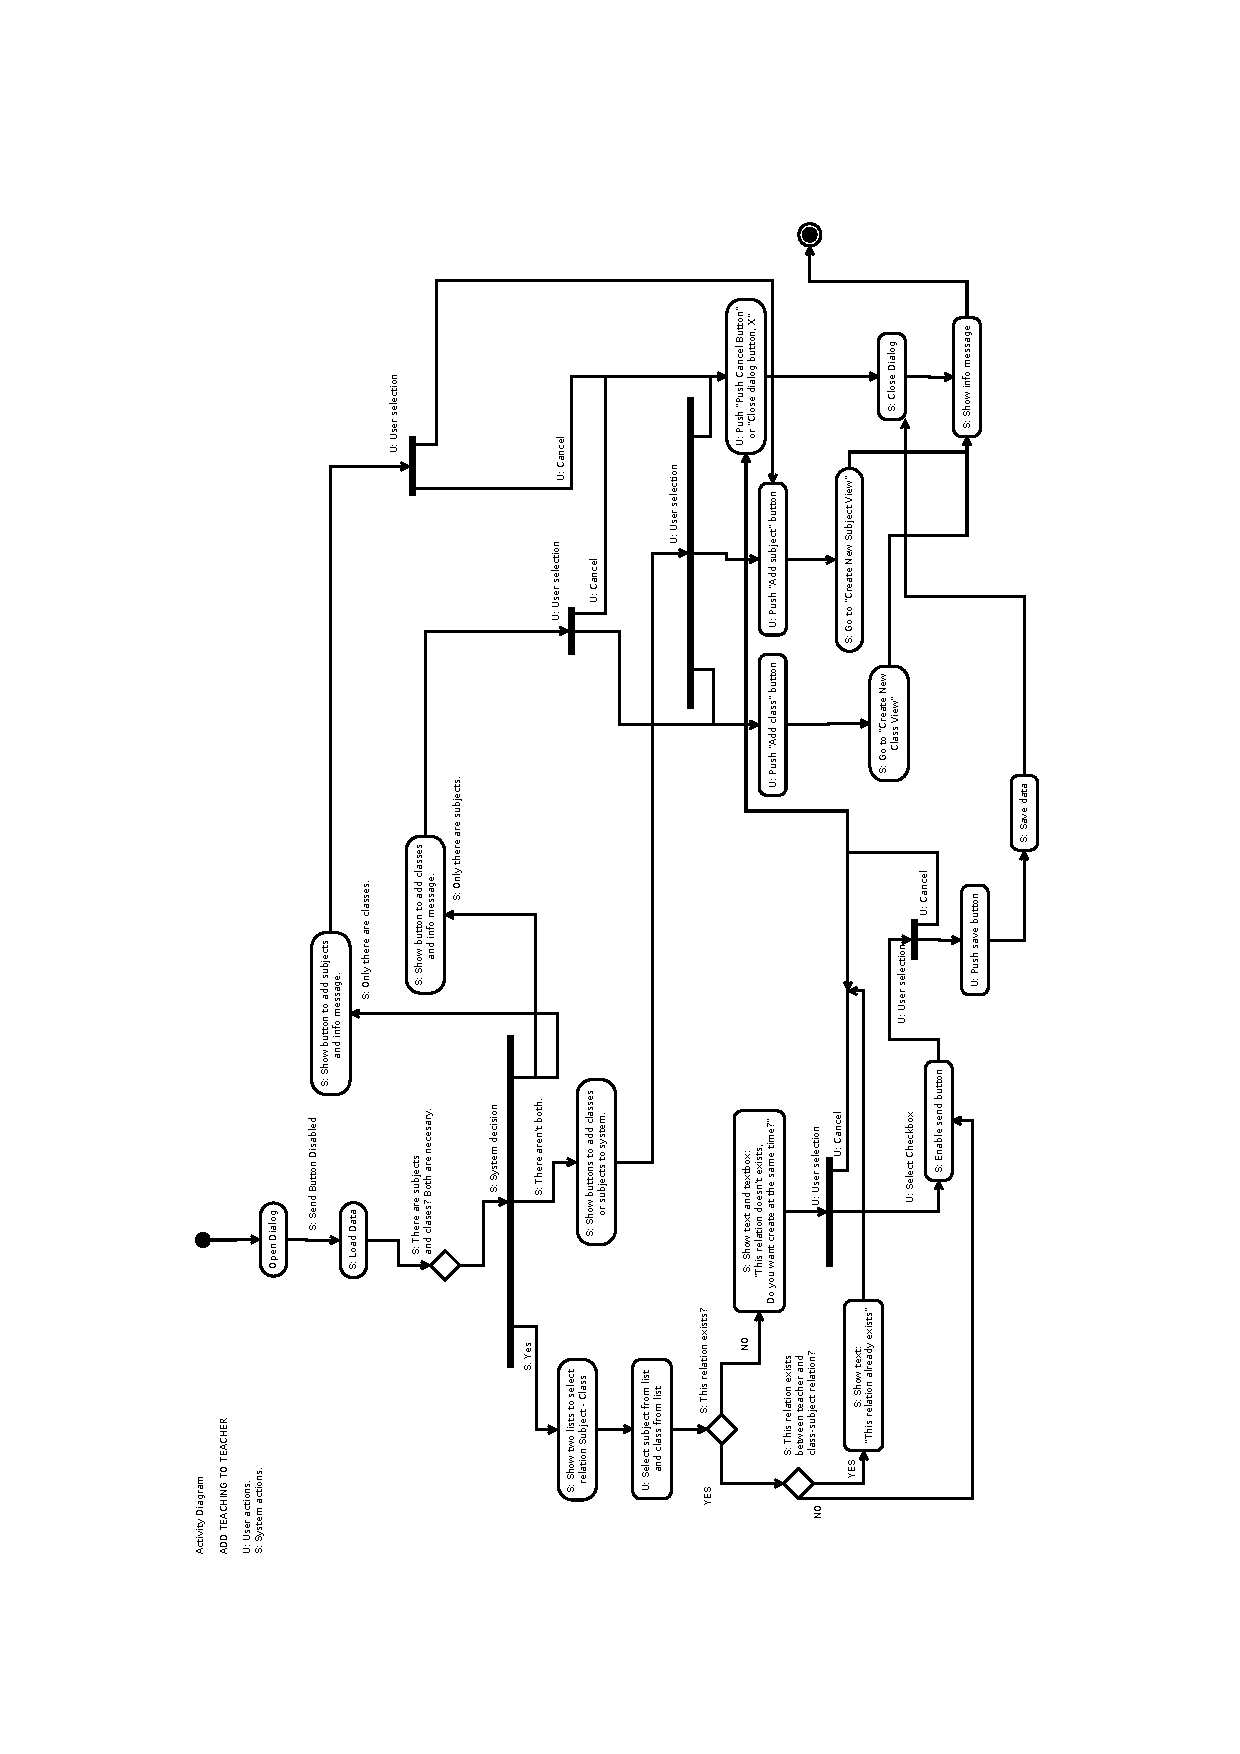
\includepdf[pages=-,pagecommand={},scale=0.94]{img/diagrams/addTeachingToTeacher_AD.pdf}

% \begin{figure}[H]
%   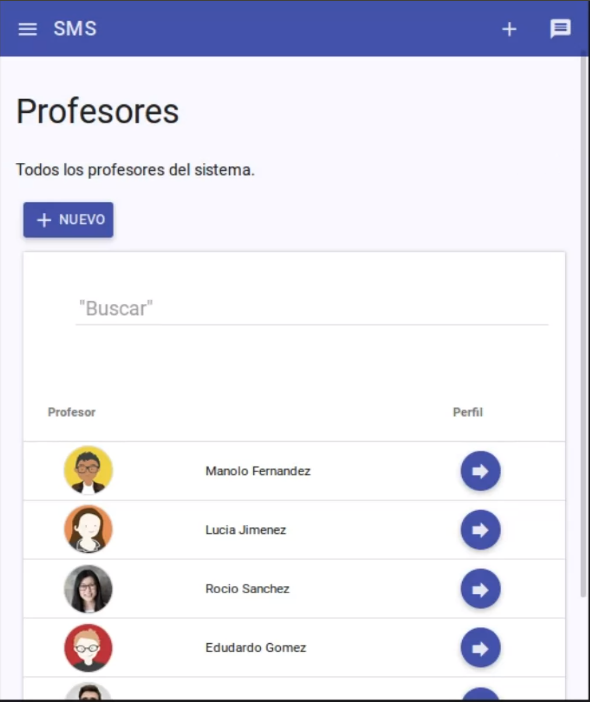
\includegraphics[scale=0.2]{img/snaps/teachers_list.png}
%   \centering
%   \caption{Teachers List view wireframed.}
% \end{figure}
%
% \begin{figure}[H]
%   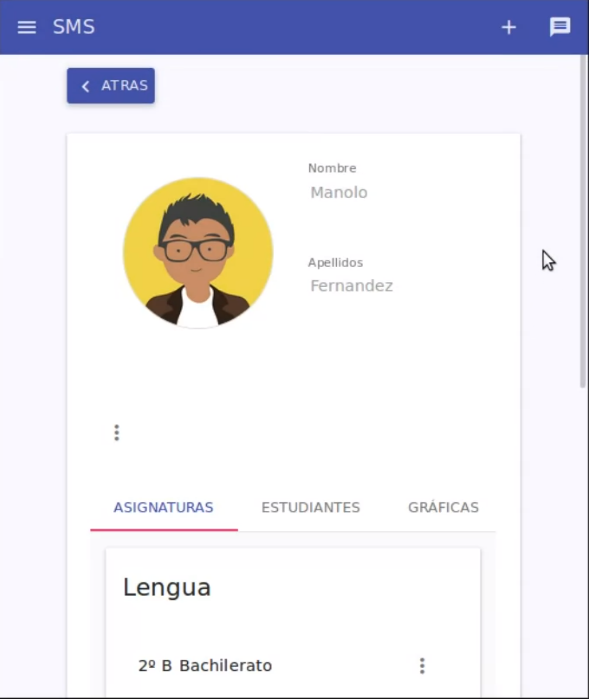
\includegraphics[scale=0.2]{img/snaps/teacher_profile.png}
%   \centering
%   \caption{Teachers List view wireframed.}
% \end{figure}

\noindent One has been decided the design with wireframes and the interaction
with flow/activity diagrams the rest is to implement this with CSS Framework
selected and develop all logic so the system satisfies all requirements.
This is some snaps of the interface already designed.
\intro
The teacher list, where we can see a simple dynamic list to manage teachers,
where we can see basic info and can access to complete info. And can see the
material design rules applied already.

\begin{figure}[H]
\centering
\begin{minipage}{.5\textwidth}
  \centering
  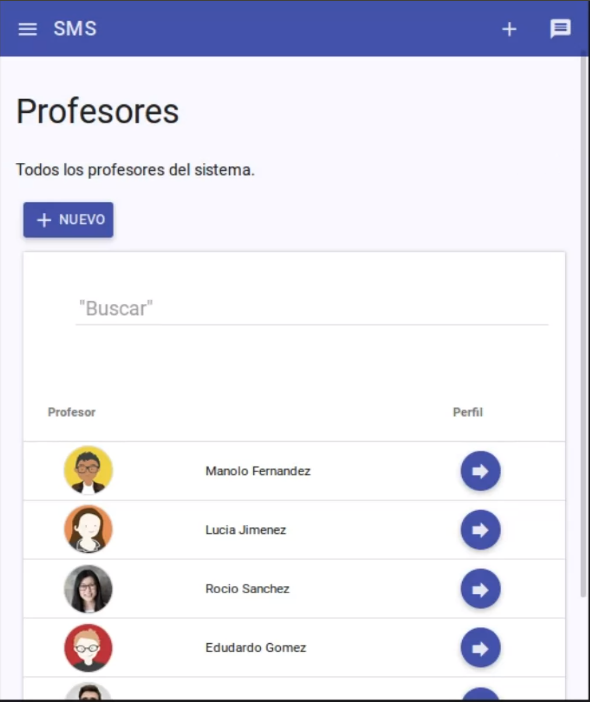
\includegraphics[scale=0.3]{img/snaps/teachers_list.png}
  \caption{A figure}
\end{minipage}%
\begin{minipage}{.5\textwidth}
  \centering
  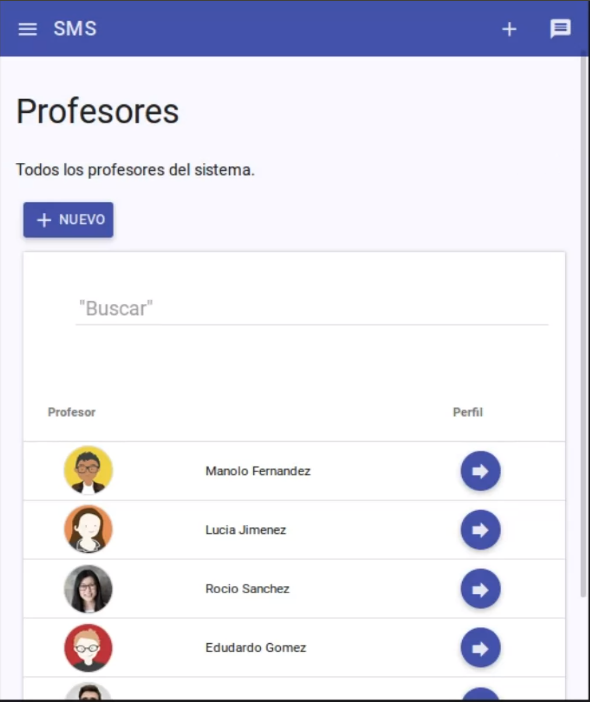
\includegraphics[scale=0.3]{img/snaps/teachers_list.png}
  \caption{Another figure}
\end{minipage}
\end{figure}

\noindent The pictures below show us teacher profile section, with
the same philosophy.

\begin{figure}[H]
\centering
\begin{minipage}{.5\textwidth}
  \centering
  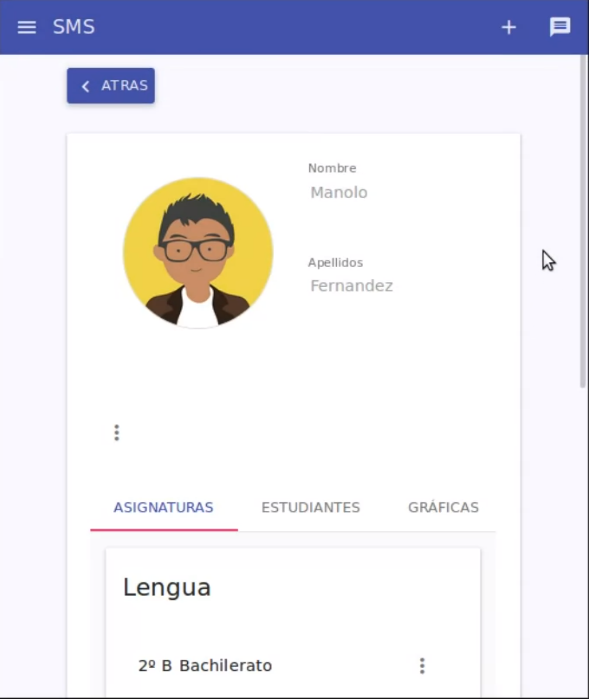
\includegraphics[scale=0.3]{img/snaps/teacher_profile.png}
  \caption{A figure}
\end{minipage}%
\begin{minipage}{.5\textwidth}
  \centering
  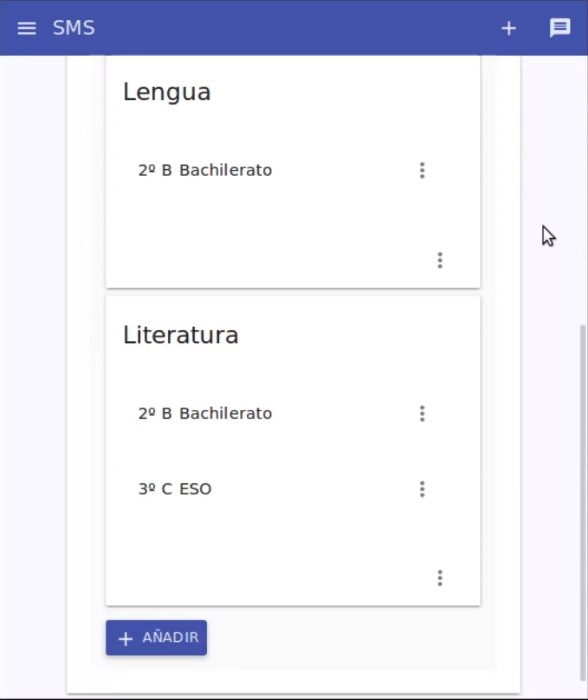
\includegraphics[scale=0.3]{img/snaps/teacher_profile_2.png}
  \caption{Another figure}
\end{minipage}
\end{figure}

\noindent Aso, for example, updating a teacher profile (note that this is
the spanish version).

\begin{figure}[H]
\centering
\begin{minipage}{.5\textwidth}
  \centering
  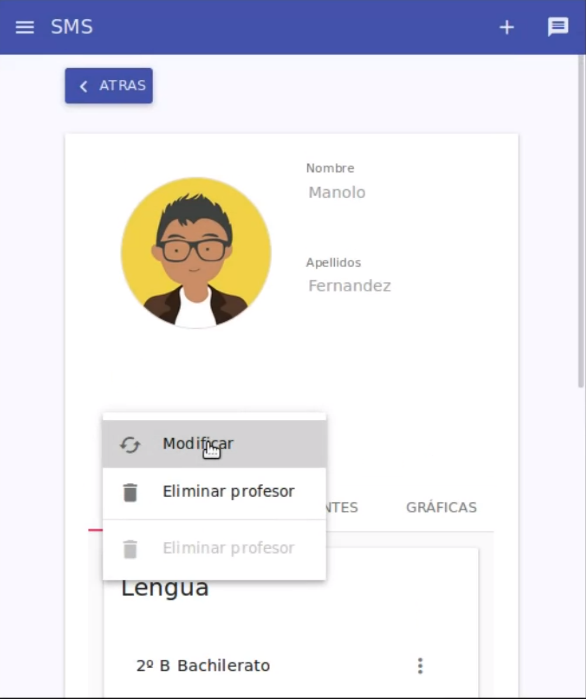
\includegraphics[scale=0.3]{img/snaps/teacher_profile_update.png}
  \caption{A figure}
\end{minipage}%
\begin{minipage}{.5\textwidth}
  \centering
  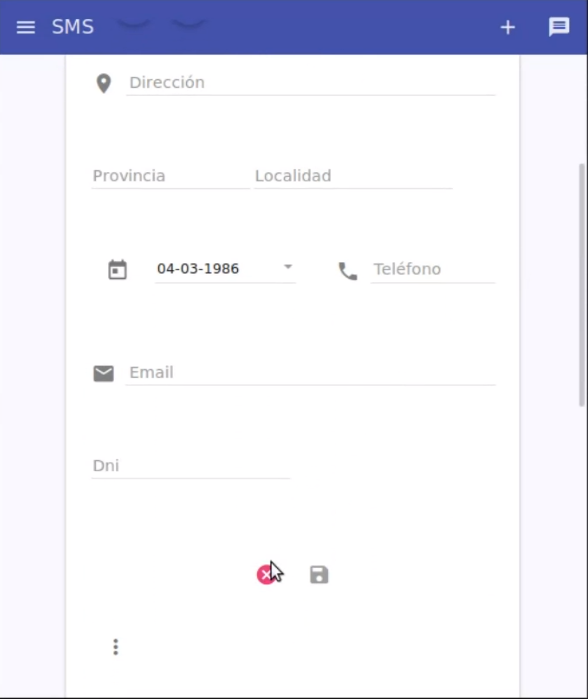
\includegraphics[scale=0.3]{img/snaps/teacher_profile_update2.png}
  \caption{Another figure}
\end{minipage}
\end{figure}

\noindent Now, students list view and some graphics.

\begin{figure}[H]
\centering
\begin{minipage}{.5\textwidth}
  \centering
  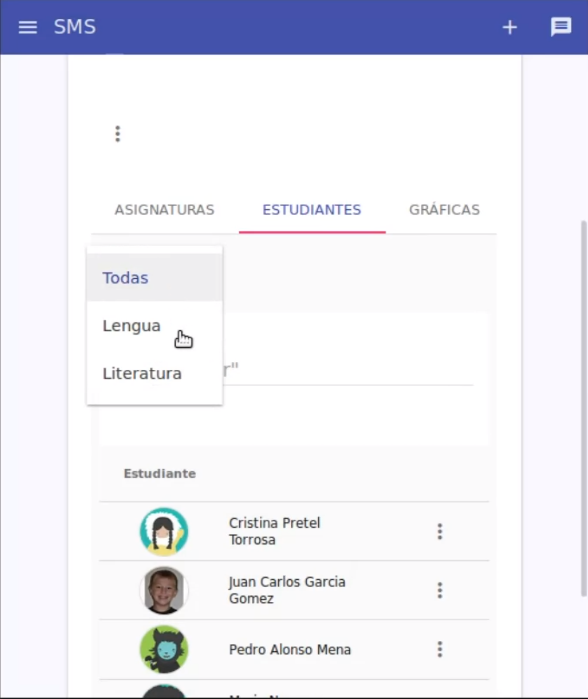
\includegraphics[scale=0.3]{img/snaps/teacher_profile_students.png}
  \caption{A figure}
\end{minipage}%
\begin{minipage}{.5\textwidth}
  \centering
  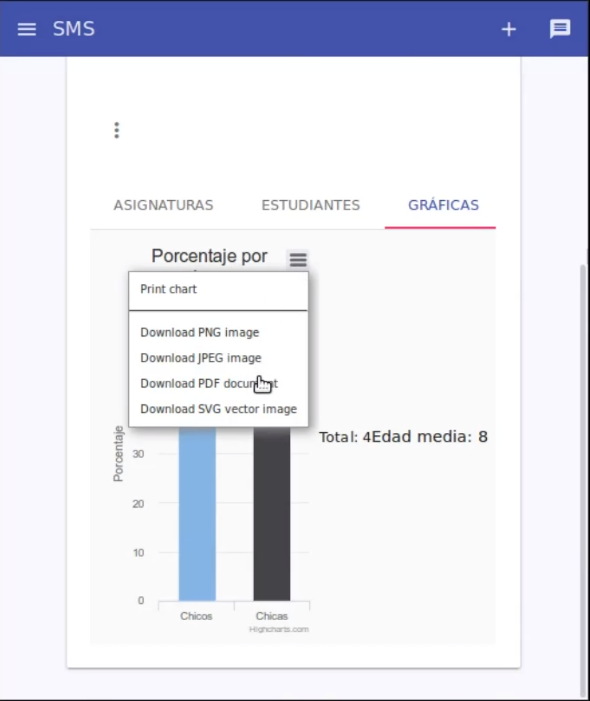
\includegraphics[scale=0.3]{img/snaps/teacher_profile_graphics.png}
  \caption{Another figure}
\end{minipage}
\end{figure}

\noindent And the rest of app follow the same look and feel, responsive and well adaptable
for almost any device.

\section{Analysis microService}

In the case of this service, the developing not have gone too far and only have
been implemented some simple linear regressions to can give a simple way to
predict the future values of some data block, as student marks or their efficiency
(as we have discussed already).

In conclusion, this service will offer mocks of all data expected and will be
the main goal in futures sprints of the project.
